\chapter{Expectation Maximization}
\label{ch-emax}

This chapter is based on 
Refs.\cite{wiki-em}
and \cite{emory-biostat}.

The Expectation Maximization (EM) 
algorithm 
is commonly used in Data Science 
to find the maximum
over an {\bf unknown parameter} $\theta$ of a
 likelihood function 

\beq
P(\vecx|\theta)=
\sum_\vech P(\vecx, \vech|\theta)
\;,
\eeq
where $\vecx$
denotes the {\bf observed variables},
and $\vech$ denotes the
{\bf latent variables}.
Both $\theta$
and $\vech$
are hidden (i.e.,
unobserved).\footnote{
The term
``unknown parameter"
is frequentist lingo.
For Bayesians, $\theta$
is a random variable with
a delta function prior,
whereas for frequentists,
it is not
a random variable at all, 
just an unknown parameter
with no randomness.}



\begin{figure}[h!]
\centering
$$\begin{array}{ccc}
\xymatrix{
\ul{\theta}\ar[d]\ar[dr]
\\
\ul{\vecx}&\ul{\vech}\ar[l]
}
&=&
\xymatrix{
\ul{\theta}
\ar[d]
\ar@/_1pc/[dd]
\ar@/_1pc/[ddd]
\ar[rd]\ar[rdd]\ar[rddd]
\\
\rvx[0]
&\rvh[0]\ar[l]
\\
\rvx[1]
&\rvh[1]\ar[l]
\\
\rvx[2]
&\rvh[2]\ar[l]
}
\end{array}
$$
\caption{bnet for EM with $nsam=3$.}
\label{fig-em-bnet}
\end{figure}


The bnet for the EM algorithm
is given by Fig.\ref{fig-em-bnet}
for $nsam=3$.
Later on in this chapter,
we will give the node TPMs
for this bnet for
the special
case in which $P(x[i]\cond \theta)$
is a mixture (i.e., weighted sum)
of Gaussians.

Note that if we 
erase the $\rvh[i]$ nodes
from Fig.\ref{fig-em-bnet},
we get the bnet for naive Bayes,
which is used for classification
into the states of $\ul{\theta}$.
However, there is one big
difference. 
With naive Bayes,
the leaf nodes have
different TPMs.
Here, we will assume they are i.i.d.
Naive Bayes is used for classification: i.e., 
given the states 
of the leaf nodes,
we infer the state of the root node.
EM is used for clustering; i.e.,
given many i.i.d. samples,
we fit their distribution by a weighted sum
of prob distributions,
usually Gaussians.

Let
 
$\call=$likelihood 
function.

$nsam=$ number of samples.

$\vecx=(x[0], x[1], \ldots, x[nsam-1])$ =
{\bf observed data}.
 $x[i]\in S_\rvx$ for all $i$.

$\vech=(h[0], h[1], \ldots, h[nsam-1])$
= {\bf hidden or missing data}.
$h[i]\in S_\rvh$ for all $i$.

We assume that the samples $(x[i],h[i])$
are i.i.d. for different $i$ at fixed 
$\theta$.
What this means is that 
there are
probability distributions
$P_{\rvx|\rvh,\ul{\theta}}$
and $P_{\rvh|\ul{\theta}}$
such that

\beq
P(\vecx, \vech|\theta)=
\prod_i \left[P_{\rvx|\rvh,\ul{\theta}}
(x[i]\cond h[i], \theta)
P_{\rvh|\ul{\theta}}(h[i]\cond \theta)\right]
\;.
\eeq

Definition of likelihood functions:
\beqa
\underbrace{P(\vecx|\theta)}
_{\call(\theta;\vecx)}
&=&
\sum_{\vech}
\underbrace{P(\vecx,\vech|\theta)}
_{\call(\theta;\vecx,\vech)}
\eeqa


$\theta^*=$ maximum likelihood
estimate of $\theta$ (no prior $P(\theta)$
assumed):

\beq
\theta^*=
\argmax_\theta\call(\theta;\vecx)
\eeq

\hrule\noindent
{\bf The EM algorithm:}
\begin{enumerate}
\item{\bf Expectation step:} 
\beq
Q(\theta|\theta^{(t)})
=
E_{\vech|\vecx,\theta^{(t)}}\ln P(\vecx,\vech|\theta)
\label{eq-exp-step}
\eeq

\item{\bf Maximization step:}

\beq
\theta^{(t+1)}=\argmax_\theta
Q(\theta|\theta^{(t)})
\eeq
\end{enumerate}
Claim: $\lim_{t\rarrow \infty}
\theta^{(t)}=\theta^*$.

\begin{figure}[h!]
$$\xymatrix{
\ul{\theta}^{(0)}\ar[d]\ar[dr]\ar[r]
&\ul{\theta}^{(1)}\ar[r]
&\ul{\theta}^{(2)}\ar[r]
&\cdots\theta^*
\\
\ul{\vecx}\ar[ru]\ar[rru]\ar[urrr]
&\ul{\vech}\ar[l]
}$$
\caption{
The EM algo generates 
a sequence of 
parameter estimates 
$(\theta^{(t)})_{t=0, 1,2, \ldots}$
that converges to the optimum (i.e., 
best-fit) parameter $\theta^*$.
}
\label{fig-emax-dynamical-bnet}
\end{figure}

Fig.\ref{fig-emax-dynamical-bnet}
portrays the 
recursive nature of 
the EM algo as a dynamical, recurrent bnet.
For Fig.\ref{fig-emax-dynamical-bnet},
the TPMs, printed in blue,
for the
$\ul{\theta}^{(t)}$
nodes for $t=1, 2, \ldots$, are
as follows:

\beq\color{blue}
P(\theta^{(t+1)}|\vecx, \theta^{(t)})=
\delta(\theta^{(t+1)}, \argmax_\theta
 Q(\theta|\theta^{(t)}))
\;.
\eeq

\hrule
\section*{Motivation}

\beqa
Q(\theta|\theta^{(t)})
&=&
E_{\vech|\vecx,\theta^{(t)}}
\ln P(\vecx,\vech|\theta)
\\
&=&
E_{\vech|\vecx,\theta^{(t)}}[
\ln P(\vech|\vecx, \theta) 
+\ln P(\vecx|\theta)]
\\
&=&
-D_{KL}\left(
P(\vech|\vecx, \theta^{(t)}) 
\parallel
P(\vech|\vecx, \theta)
\right) 
-H[P(\ul{\vech}|\vecx, \theta^{(t)})]
+\ln P(\vecx|\theta)
\label{eq-Q-decomposed}
\eeqa
When $\theta^{(t)}=\theta$,
this becomes

\beq
Q(\theta|\theta)=
-H[P(\ul{\vech}|\vecx, \theta)]+
\ln P(\vecx|\theta)
\;.
\eeq
Hence, 

\beqa
\partial_\theta Q(\theta|\theta)
&=&
-\sum_{\vech}\partial_\theta
P(\ul{\vech}|\vecx, \theta)
+
\partial_\theta
\ln P(\vecx|\theta)
\\
&=&
\partial_\theta
\ln P(\vecx|\theta)
\eeqa

So if $\theta^{(t)}\rarrow \theta$
and $Q(\theta|\theta)$ is max at $\theta=\theta^*$,
then $\ln P(\vecx|\theta)$
is max at $\theta=\theta^*$ too.

For a  more rigorous proof
that $\lim_{t\rarrow \infty}\theta^{(t)}
=\theta^*$,
see Wikipedia article Ref.\cite{wiki-em}
and references therein.

\section*{Minorize-Maximize (MM) algorithms}


\begin{figure}[h!]
\centering
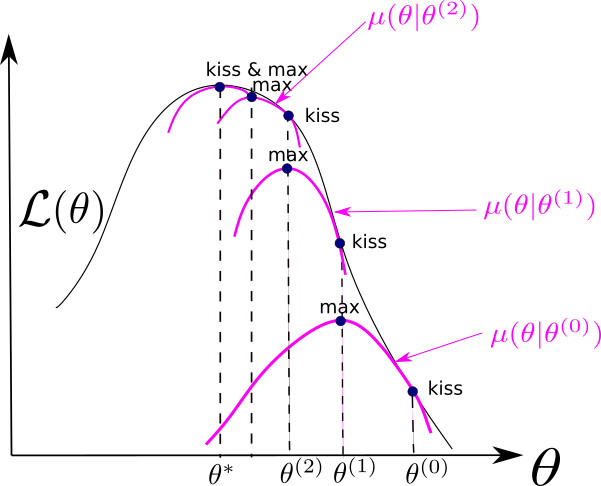
\includegraphics[width=3.7in]
{emax/minorize.png}
\caption{Function $\mu(\theta|\theta^{(t)})$
minorizes the function $\call(\theta)$.
Note that $\mu(\theta|\theta^{(t)})$
is always below
 $\call(\theta)$.
``max" indicates 
$\theta^{(t+1)}=
\argmax_\theta \mu(\theta|\theta^{(t)})$.
``kiss" indicates
 $\mu(\theta^{(t)}|\theta^{(t)})=
\call(\theta^{(t)})$. 
}
\label{fig-minorize}
\end{figure}



A function {\bf $\mu(\theta|\theta^{(t)})$ 
is said to minorize 
 a target
 function $\call(\theta)$}
iff for all $ \theta$ at fixed 
$\theta^{(t)}$,
it satisfies the
``$\mu\leq\call$ property"


\beq
\mu(\theta|\theta^{(t)})\leq
\call(\theta)
\;,
\eeq
and
the ``$\mu=\call$ property"

\beq
\mu(\theta^{(t)}|\theta^{(t)})=
\call(\theta^{(t)})
\;.
\eeq

We  {\bf recursively maximize a minorizing function} $\mu(\theta|\theta^{(t)})$
if we define a sequence $(\theta^{(t)})_{t=0, 1, \ldots}$
as follows:

\beq
\theta^{(t+1)}=\argmax_\theta \mu(\theta|\theta^{(t)})
\;.
\eeq

The sequence 
$(\call(\theta^{(t)}))_{t=0, 1, 2, \ldots}$
generated by 
recursively maximizing a minorizing function
must be nondecreasing:

\beq
\call(\theta^{(t+1)})\geq \mu(\theta^{(t+1)}
|\theta^{(t)})\geq
 \mu(\theta^{(t)}|\theta^{(t)}) 
= \call(\theta^{(t)})
\;.
\eeq

A {\bf
minorize-maximize (MM) algorithm}
is any algo that
specifies a
minorizing function $\mu(\theta|\theta^{(t)})$
for a particular target
 function $\call(\theta)$.
One can also define a 
{\bf majorize-minimize algo (also
called  MM)}
by inverting the inequalities throughout.


The EM algo is an MM algo.
Indeed, if we define 

\beq
\call(\theta)=\ln P(\vecx|\theta)
\eeq
and

\beq
\mu(\theta|\theta^{(t)})
=
Q(\theta|\theta^{(t)})
+
H(P(\ul{\vech}|\vecx, \theta^{(t)})
\;,
\eeq
then Eq.(\ref{eq-Q-decomposed})
establishes
the $\mu\leq \call$
and $\mu=\call$ properties
required of 
a minorizing function.

How an MM algo works 
is portrayed in Fig.\ref{fig-minorize}.


\section*{Examples}

\hrule\noindent{\bf Example (Gaussian mixture)}


$x[i]\in \RR^d=S_\rvx$. $S_\rvh$ discrete and
not too large. $n_\rvh=|S_\rvh|$ is
number of Gaussians that we are 
going to fit the samples with.

Let
\beq
\theta = [w_h, \mu_h, \Sigma_h]_{h\in S_\rvh}
\;,
\eeq
where
$[w_h]_{h\in S_\rvh}$ is a probability
distribution of weights, and 
where $\mu_h\in\RR^d$
and $\Sigma_h\in\RR^{d\times d}$
are the mean value vector 
and covariance matrix of
a $d$-dimensional Gaussian distribution.

The TPMs, printed in blue,
for the nodes of Fig.\ref{fig-em-bnet},
for the special case
of a mixture of Gaussians, are as follows:

\beq\color{blue}
P(x[i]\cond h[i]\cond \theta)=
\caln_d(x[i];\mu_{h[i]}, \Sigma_{h[i]})
\eeq

\beq\color{blue}
P(h[i]\cond \theta)=w_{h[i]}
\eeq

Note that

\beqa
P(x[i]\cond \theta)&=&
\sum_h P(x[i]\cond h[i]=h, \theta)
P(h[i]=h\cond\theta)
\\
&=&
\sum_hw_h\caln_d(x[i];\mu_h, \Sigma_h)
\eeqa

\beqa
P(\vecx, \vech|\theta)&=&
\prod_i \left[
w_{h[i]}
\caln_d(x[i];\mu_{h[i]}, \Sigma_{h[i]})
\right]
\\
&=&
\prod_i\prod_h
\left[w_h
\caln_d(x[i];\mu_h, \Sigma_h)\right]
^{\indi(h=h[i])}
\eeqa

{\bf Old Faithful:}
See Wikipedia Ref.\cite{wiki-em}
for an animated
gif of a  classic example
of using EM to fit
samples with a Gaussian mixture.
Unfortunately,
could
not include it
here because pdflatex
does not support animated gifs. 
The gif shows samples in a 2 dimensional
space
(eruption time, delay time)
from the Old Faithful geyser.
In that example, $d=2$ and $n_\rvh=2$.
Two clusters of points
in a plane are fitted
by 
a mixture of 2 Gaussians.

{\bf K-means clustering} is often
presented as the main competitor
to EM for doing 
{\bf clustering (non-supervised
learning)}. In K-means clustering,
the sample points are 
split into $K$
mutually
disjoint sets $S_0, S_1, \ldots, S_{K-1}$. 
The algorithm is easy
to describe:
\begin{enumerate}
\item
Initialize by 
choosing  at random
$K$ data points $(\mu_k)_{k=0}^{K-1}$
called means or centroids
and placing $\mu_k$ in $S_k$
for all $k$.
 \item {\bf STEP 1:}
For each data point,
add it to the $S_k$
whose centroid $\mu_k$
is closest to it.
\item {\bf STEP 2:}
Recalculate the centroids.
Set $\mu_k$ equal to the mean value of set
$S_k$.
\item Repeat steps 1 and 2 until the
centroids stop changing 
by much.
\end{enumerate}
Step 1 is analogous
to the expectation step in EM,
and Step 2 to the maximization
step in EM ($\theta$
estimation versus 
$\mu_k$ estimation).
We won't say anything further
about K-means clustering because
it
isn't related to bnets in any 
way, and this is a book about bnets.
For more info about
K-means clustering, 
see Ref.\cite{wiki-k-means}.

\hrule\noindent{\bf
 Example (Blood Genotypes and Phenotypes):}

Notation:
$\vec{\rva}=
(\rva[\sigma])_{\sigma=0, 1, \ldots,nsam-1}
$, where $nsam$
is the number of samples.
Will
sometimes
denote
$a\sqsig$ by $a^\sqsig$.


Suppose
$\vec{\rvx}=
(\vec{\rvx}_0)
$ (i.e., just one component)

$\vec{\rvh}=
(\vec{\rvh}_0)
$ (i.e., just one component)



$\rvh[\sigma]\in S_\rvh=
\{AA, AO, BB, BO, OO, AB\}$ (the 6 blood genotypes)

$\rvx[\sigma]\in S_\rvx=
\{A,B,O,AB\}$ (the 4 blood phenotypes)

\begin{figure}[h!]
$$
\xymatrix{
\ul{\theta}\ar[d]\ar[dr]
\\
\rvx[\sigma]&\rvh[\sigma]\ar[l]
}$$
\caption{bnet 
for blood phenotypes $x\sqsig$
and genotypes $h\sqsig$.}
\label{fig-phenotypes}
\end{figure}

For the bnet of Fig.\ref{fig-phenotypes},
the TPMs, printed in blue, are:
\beq\color{blue}
P(h^\sqsig| \theta)=
\begin{array}{c|c}
&
\\\hline
AA&p_A^2
\\
AO&2p_Ap_O
\\
BB&p_B^2
\\
BO&2p_Bp_O
\\
OO&p_O^2
\\
AB&2p_Ap_B
\end{array}
\;,
\label{eq-pheno-ph}
\eeq
where $p_A+p_B+p_O=1$.


\beq\color{blue}
P(x^\sqsig\cond h^\sqsig, \theta)=
\begin{array}{l|llllll}
&AA&AO&BB&BO&OO&AB
\\\hline
A&1&1&0&0&0&0
\\
B&0&0&1&1&0&0
\\
O&0&0&0&0&1&0
\\
AB&0&0&0&0&0&1
\end{array}
\label{eq-pheno-pxbarh}
\eeq

\beq
\theta=(p_A, p_B)
\eeq

Multiplying the TPMs in
Eqs.(\ref{eq-pheno-ph}
and (\ref{eq-pheno-pxbarh}), we get
\beq
P(x^\sqsig\cond \theta)=
\begin{array}{l|l}
\\\hline
A&p_A^2+2p_Ap_O(=\pi_A)
\\
B&p_B^2+2p_Bp_O(=\pi_B)
\\
O&p_O^2(=\pi_O)
\\
AB&2p_Ap_B(=\pi_{AB})
\end{array}
\eeq


Note that 
\beqa
P(\vec{x}|\theta)
&=&
\prod_\sigma
P(x^\sqsig|\theta)
\\
&=&
(\pi_A)^{N_A}
(\pi_B)^{N_B}
(\pi_O)^{N_O}
(\pi_{AB})^{N_{AB}}
\;,
\eeqa 
where 
$N_x$ for $x\in S_\rvx=\{A, B, O, AB\}$
are
the counts from the data.
We can get estimates
for the parameters $p_A$ and $p_B$
right
here without doing EM.
Just note that

\beq
\hat{\pi}_x=
\frac{N_x}
{N_+}
\label{eq-quads-pi-x}
\eeq
for $x\in S_\rvx$,
where
$N_+=\sum_x N_x$. 
Eqs.(\ref{eq-quads-pi-x})
give  4 quadratic equations
that can be solved for the
parameters $p_A, p_B$
in terms of the observed 
counts $N_x$
for $x\in S_\rvx$.


If, instead,  you want to
find the optimum
parameters $p_A, p_B$
using EM, note that

\beqa
Q(\theta|\theta^{(t)})
&=&
\sum_{\vec{h}}
P(\vec{h}|\theta^{(t)})
\ln P(\vec{x}, \vec{h}|\theta)
\\
&=&
\sum_{\vec{h}}
\left[\prod_\sigma
P(h^\sqsig|\theta^{(t)})
\right]
\ln \left[
\prod_\sigma P(x^\sqsig, h^\sqsig |\theta)
\right]
\\
&=&\sum_\sigma 
\sum_{h^\sqsig}
P(h^\sqsig|\theta^{(t)})
\ln
 P(x^\sqsig, h^\sqsig |\theta)
\\
&=&\sum_\sigma 
\sum_{h^\sqsig}
P(h^\sqsig|\theta^{(t)})
[\ln
 P(x^\sqsig| h^\sqsig ,\theta)
+
\ln
 P(h^\sqsig |\theta)
]
\\
&=&nsam 
\sum_{h^\sqsig}
P(h^\sqsig|\theta^{(t)})
\ln
 P(h^\sqsig |\theta)
\;.
\eeqa

\hrule\noindent{\bf
 Example (Missing Data/Imputation):}

The previous example
on blood genotypes and phenotypes
assumed no missing
data in compiling the
counts $N_x$. 
But what if there is missing
data? Can one
still apply
the EM algo in that case?
Yes! See Chapter \ref{ch-missing-d}.


